In den Kapiteln \ref{Controller-Dispatcher-UseCase-Interactor} und \ref{Port-Adapter-Controller} 
werden die fertigen Strukturen beschrieben, diese Strukturen müssen am Anfang des Programms erstellt
und miteinander verbunden werden.

Das Erstellen von der Struktur findet im Hauptprogramm statt und lässt sich in drei Schritte aufteilen:
\begin{itemize}
    \item Erstellen alle Instanzen
    \item Verknüpfen alle Instanzen miteinander
    \item Starten alle Instanzen
\end{itemize}

Das Erstellen aller Instanzen lässt sich in zwei weitere Schritte aufteilen, die bedingt voneinander abhängen.
\begin{itemize}
    \item Kern (Controllers + Dispatcher + UseCases + Interactors)
    \item Schnittstellen (Port + Adapter + Controller)
\end{itemize}

Damit auch Integrationstests für den kompleten Core und jede Schnittstellen möglich sind, wäre es sinnvol, dass beide Schritte
explicit ausgeführt werden.

Ein möglicher Ablauf wäre:
\begin{figure}[H]
    \centering
    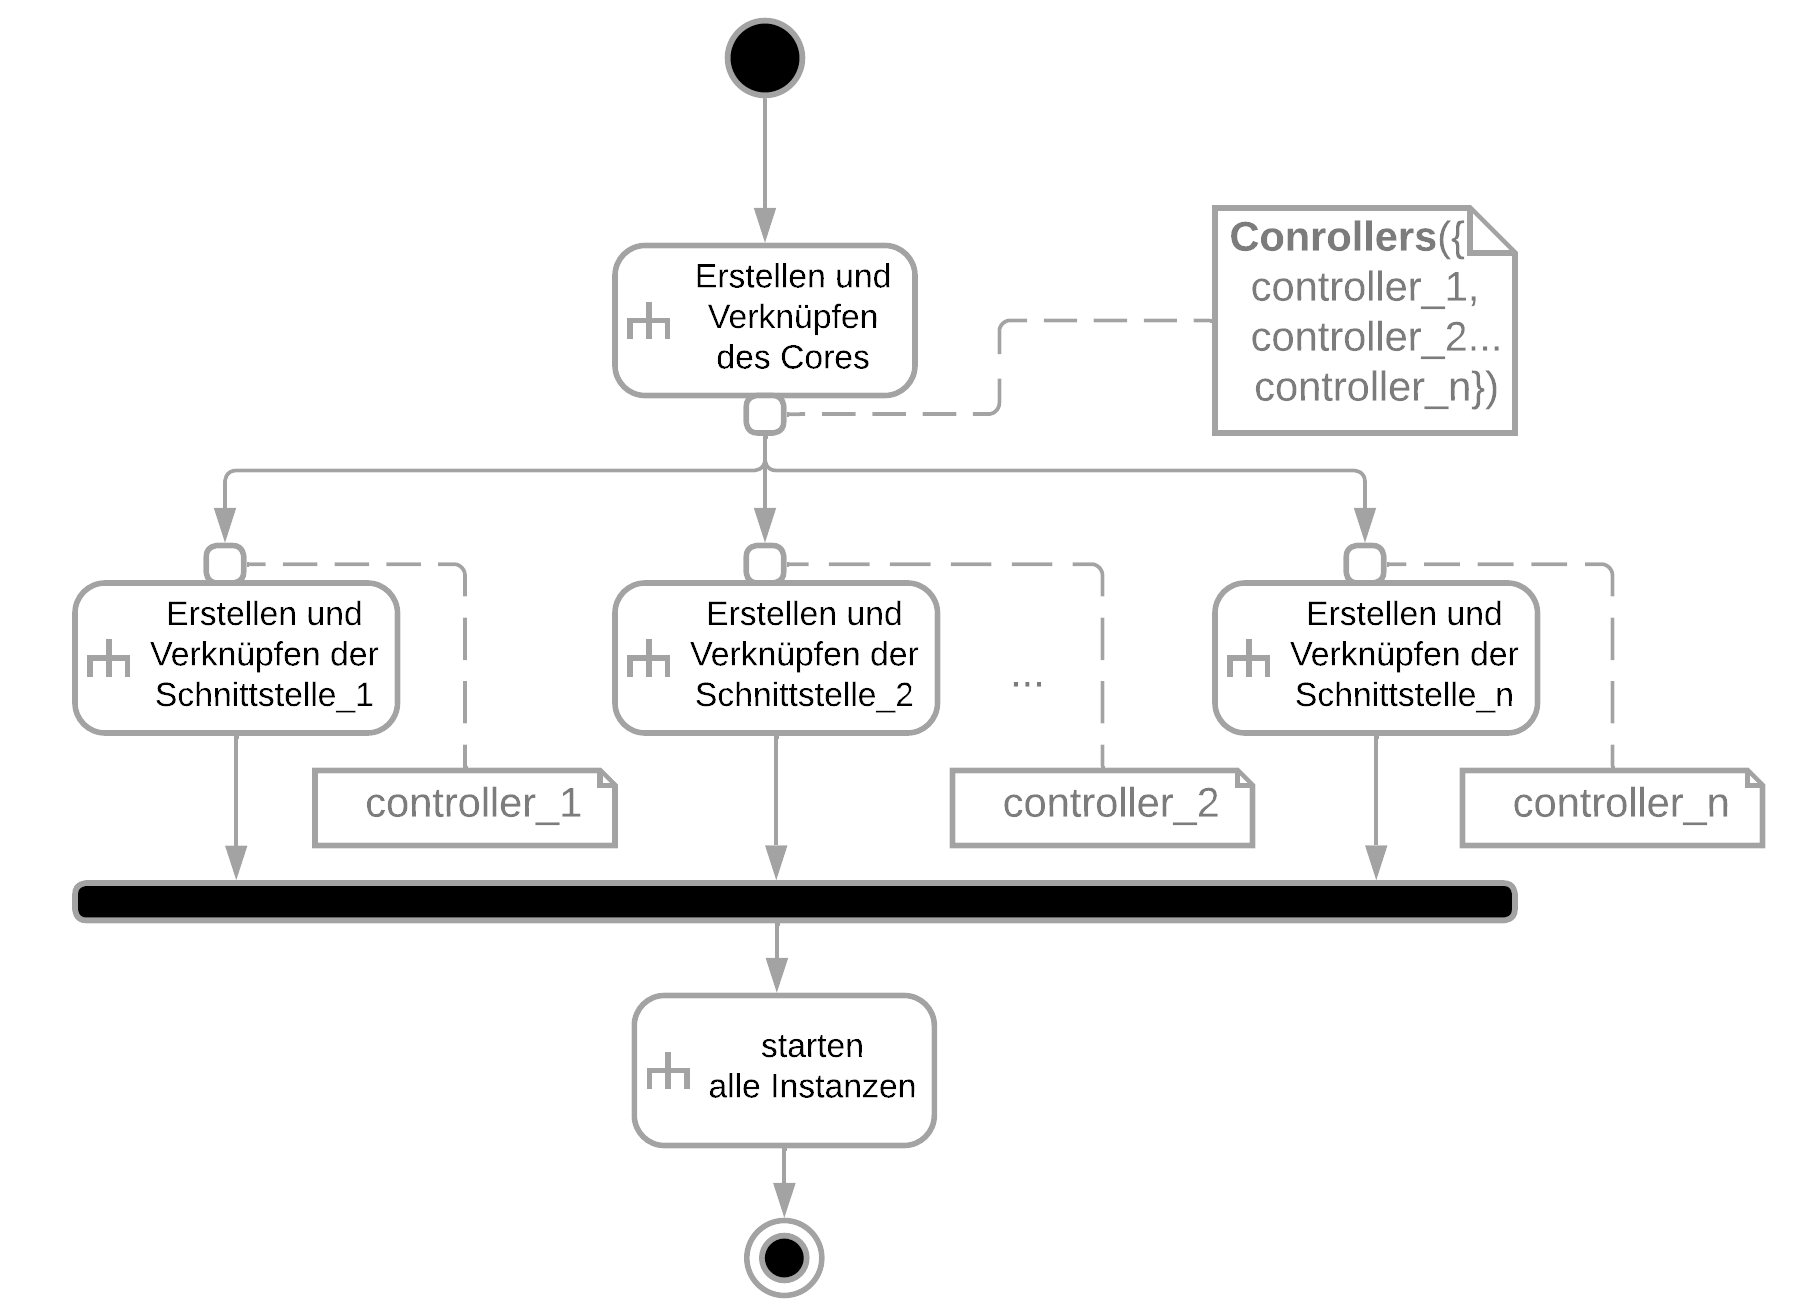
\includegraphics[width=12cm]{./images/Erstellen AD.png}
     \caption[Ablaufiagramm Erstellen der Struktur]{Ablaufiagramm Erstellen der Struktur \footnotemark}
     \label{fig:ADCreate}
\end{figure}

Mit diesem Ablauf können mehrere Hauptprogramme erstellt werden, die verschiedene Anwendungen für verschiedene Zwecke erstellen.
Z.B. ein Framework braucht keine reelen Anknüpfungen an die Infrastruktur (z.B. Datenbank) im Vergleich zu Standalone Anwendung.
Oder es können verschiedene Hauptprogramme für verschiedene Datenbanken geben.
